\documentclass{jlreq}
\usepackage{graphicx,tcolorbox}
\usepackage{mathtools,diffcoeff,unicode-math}
\setmathfont{NewComputerModernMath}
\newtcolorbox{hako}[1]{colframe=black,colback=white,coltitle=black,colbacktitle=white,boxrule=0.8pt,arc=0mm,title={\textbf{#1}},}
\usepackage[thicklines]{cancel}
\usepackage[hidelinks]{hyperref}
\usepackage{tikz}
\usetikzlibrary{calc, arrows.meta}
\usepackage{wrapfig}
\setlength{\parindent}{0pt}
\usepackage[normalem]{ulem}
\pagestyle{empty}
\usepackage[dvipsnames]{xcolor}
\definecolor{darkred}{RGB}{150, 0, 0}
\definecolor{darkblue}{RGB}{0, 0, 150}
% \newcommand{\akairo}[1]{\textcolor{BrickRed}{\underline{#1}}}
% \newcommand{\aoiro}[1]{\textcolor{RoyalBlue}{\underline{#1}}}
\newcommand{\akairo}[1]{{\color{darkred}\underline{{\color{black}#1}}}}
\newcommand{\aoiro}[1]{{\color{darkblue}\underline{{\color{black}#1}}}}
\begin{document}
\begin{flushleft}
    \Large\textbf{Euler-Lagrange eqationを用いた回転座標系の運動方程式}
\end{flushleft}
\vspace{0.5\baselineskip}
\begin{wrapfigure}{r}{60mm}
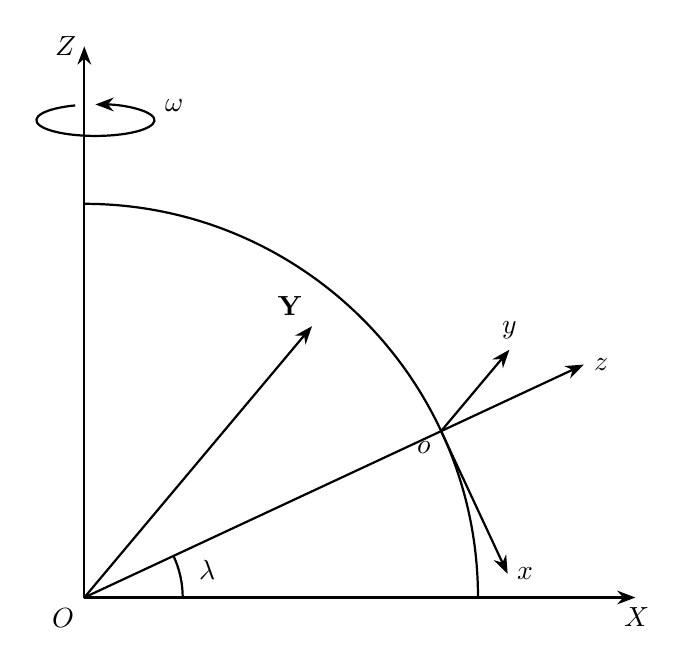
\begin{tikzpicture}[>=Stealth, scale=5, thick]
    % --- 座標定義 ---
    \coordinate (O) at (0,0);
    \def\lat{25} % 緯度角 lambda
    \coordinate (P) at (\lat:1); % 局所座標系の原点(円弧上の点)
    
    % --- 1. Z軸を長く取り,omega と円弧を離す ---
    % Z軸
    \draw[->] (0,0) -- (0,1.4) node[left] {$Z$};
    % X軸
    \draw[->] (0,0) -- (1.4,0) node[below] {$X$};
    % 原点ラベル
    \node[below left] at (O) {$O$};
    
    % 地表の円弧(半径 1.0)
    \draw (1,0) arc (0:90:1);
    
    % --- 2. Y軸と y軸を平行にする ---
    % Y軸(中心から出るベクトル.ここでは北方向を示す接線方向と同じ角度で描画)
    \def\tangentangle{\lat+25}
    \draw[->] (O) -- (\tangentangle:0.9) node[above left] {$\mathbf{Y}$};
    
    % --- 緯度角 lambda ---
    \draw (0.25,0) arc (0:\lat:0.25);
    \node at (\lat/2:0.32) {$\lambda$};
    
    % --- 3. xyz系の原点を円弧上に配置 ---
    % 地心からの線(z軸の延長線)
    \draw (O) -- (P);
    
    % 局所系の原点に o を設置
    \node[below left] at (P) {$o$};

    % z軸 (天頂方向: OからPを通る直線の延長)
    \draw[->] (P) -- ($(P) + (\lat:0.4)$) node[right] {$z$};
    
    % y軸 (北方向: P点における接線方向.Y軸と平行)
    \draw[->] (P) -- ($(P) + (\tangentangle:0.27)$) node[above] {$y$};
    
    % x軸 (東方向: 右下へ向かう方向.z, yと直交するように配置)
    \draw[->] (P) -- ($(P) + (\lat-90:0.4)$) node[right] {$x$};

    % --- omega の描画(Z軸の上端付近に配置して円弧と被らせない) ---
    \draw[->] (-0.023, 1.25) arc (110:450:0.15 and 0.04);
    \node[right] at (0.18, 1.25) {$\omega$};

\end{tikzpicture}
\caption{回転座標系の模式図} % 必要であれば
\end{wrapfigure}

\( t=0 \)で \( XZ \)  平面と \( xy \) 平面が一致し,かつ
\( y=Y \) という条件を付けるとき,

\begin{equation}
    \begin{pmatrix}
        X\\
        Y\\
        Z
    \end{pmatrix}
    =
    \begin{pmatrix}
        \cos ωt & - \sin ωt & 0\\
        \sin ωt & \cos ωt & 0\\
        0&0&1
    \end{pmatrix}
    \begin{pmatrix}
        \sin λ &0& \cos λ\\
        0&1&0\\
        - \cos λ &0& \sin λ
    \end{pmatrix}
    \begin{pmatrix}
        x\\
        y\\
        z
    \end{pmatrix}
    \label{XYZkankei}
\end{equation}

のような関係式が成立する.
簡単のために

\begin{flalign}
    &
    \begin{pmatrix}
        x'\\
        y'\\
        z'
    \end{pmatrix}
    :=
    \begin{pmatrix}
        \sin λ &0& \cos λ\\
        0&1&0\\
        - \cos λ &0& \sin λ
    \end{pmatrix}
    \begin{pmatrix}
        x\\
        y\\
        z
    \end{pmatrix}
  \hspace{275 pt}
  \label{dkan}
\end{flalign}


とすると,式\eqref{XYZkankei}の時間微分は以下の様になる.

\begin{align}
    \begin{pmatrix}
        \dot{X}\\
        \dot{Y}\\
        \dot{Z}
    \end{pmatrix}
    =&ω
    \begin{pmatrix}
        -\sin  ωt & -\cos  ωt & 0\\
        \cos  ωt &  -\sin  ωt & 0\\
        0&0&0
    \end{pmatrix}
    \begin{pmatrix}
        x'\\
        y'\\
        z'
    \end{pmatrix}
    +
    \begin{pmatrix}
        \cos ωt & - \sin ωt & 0\\
        \sin ωt & \cos ωt & 0\\
        0&0&1
    \end{pmatrix}
        \begin{pmatrix}
        \dot{x}'\\
        \dot{y}'\\
        \dot{z}'
    \end{pmatrix}
    \notag
    \\
    =&ω
    \begin{pmatrix}
        \cos ωt & - \sin ωt & 0\\
        \sin ωt & \cos ωt & 0\\
        0&0&1
    \end{pmatrix}
    \begin{pmatrix}
        0&-1&0\\
        1&0&0\\
        0&0&0
    \end{pmatrix}
    \begin{pmatrix}
        x'\\
        y'\\
        z'
    \end{pmatrix} 
    +
    \begin{pmatrix}
        \cos ωt & - \sin ωt & 0\\
        \sin ωt & \cos ωt & 0\\
        0&0&1
    \end{pmatrix}
        \begin{pmatrix}
        \dot{x}'\\
        \dot{y}'\\
        \dot{z}'
    \end{pmatrix}
    \notag 
    \\
    =&
    \begin{pmatrix}
        \cos ωt & - \sin ωt & 0\\
        \sin ωt & \cos ωt & 0\\
        0&0&1
    \end{pmatrix}
    \begin{pmatrix}
        \dot{x}' - ωy'\\
        \dot{y}' + ωx'\\
        \dot{z}'
    \end{pmatrix} 
    \label{dashkankei}
\end{align}

式\eqref{dashkankei}において右辺にかかっている行列式は
\( 1 \) であるから,左辺の大きさと右辺の行列を掛ける前のベクトルの大きさが一致する.
以上より\( o-xyz\)系 でのラグランジアンを構成する.

\begin{align}
    &L(x,y,z, \dot{x}, \dot{y} , \dot{z},t)\notag\\
    =&
    \frac{1}{2} m ( \dot{X}^2+ \dot{Y}^2 + \dot{Z}^2) - U(x,y,z)
    \notag\\
    =&
    \frac{1}{2} m 
    \left[ 
        (\dot{x}' - ωy')^2 + (\dot{y}' + ωx')^2 + \dot{z}'^2
    \right]
    - U(x,y,z)
    \notag\\
    =&
    \frac{1}{2} m 
    \left[ 
       (\sin λ \dot{x} + \cos λ \dot{z} - ω y)^2+
       (\dot{y} + ω\sin λ x + ω \cos λ z)^2+
       (-\cos λ \dot{x} + \sin λ \dot{z})^2 
    \right]
    - U(x,y,z)
\end{align}

\( x,y,z \)それぞれについてオイラー・ラグランジュ方程式を立てる.

\begin{align}
    \diffp{L}{x}=& m ω \sin λ (\dot{y} + ω\sin λ x + ω \cos λ z) - \diffp{U}{x}\notag\\
    \diff*{\diffp{L}{x}[]}{t}
    =&
    m \left[ 
        \sin λ (\sin λ \ddot{x} + \cos λ \ddot{z} - ω \dot{y})
        - \cos λ(-\cos λ \ddot{x} + \sin λ \ddot{z})
     \right]\notag\\
    =&
    m( \ddot{x} - ω \sin λ \dot{y})\notag
\end{align}
よって
\begin{equation}
    m \ddot{x} = \akairo{2m ω \sin λ \dot{y}} + \aoiro{m ω^2 \sin λ(\sin λ x + \cos λ z)} - \diffp{U}{x}
    \label{xeq}
\end{equation}

\begin{align}
    \diffp{L}{y}=& -m ω (\sin λ \dot{x} + \cos λ \dot{z} - ω y) - \diffp{U}{y} \notag \\%ここのマイナスあってたっけ
    \diff*{\diffp{L}{\dot{y}}[]}{t}=&m( \ddot{y}+ ω \sin λ \dot{x} + ω \cos λ \dot{z})\notag
\end{align}
よって
\begin{equation}
    m \ddot{y}=\akairo{-2m ω (\sin λ \dot{x} + \cos λ \dot{z}) }- \aoiro{m ω^2 y} - \diffp{U}{y}
    \label{yeq}
\end{equation}
 
\begin{align}
    \diffp{L}{z}=& m ω \cos λ(\dot{y} + ω\sin λ x + ω \cos λ z) - \diffp{U}{z}\notag\\
    \diff*{\diffp{L}{\dot{z}}[]}{t} =& m 
    \left[ \cos λ ( \cancel{\sin λ \ddot{x}} + \cos λ \ddot{z} - ω \dot{y}) + \sin λ( \cancel{- \cos λ \ddot{x}}+ \sin λ \ddot{z})\right]\notag \\
    =&
    m \ddot{z} - 2m ω \cos λ \dot{y}\notag
\end{align}
よって
\begin{equation}
    m \ddot{z} = \akairo{2m ω \cos λ \dot{y}} + \aoiro{m ω^2 \cos λ( \sin λ x + \cos λ z) }- \diffp{U}{z}
    \label{zeq}
\end{equation}
今,
\[
    \symbfit{ω} := ω
    \begin{pmatrix}
        - \cos λ\\
        0\\
        \sin λ
    \end{pmatrix} 
\]
とすると,
式\eqref{xeq},\eqref{yeq},\eqref{zeq}をベクトルとしてまとめることができる.
\begin{equation}
    m \ddot{\symbfit{r}} = \akairo{-2 m \symbfit{ω} \times \dot{\symbfit{r}}} - \aoiro{m \symbfit{ω} \times ( \symbfit{ω} \times \symbfit{r}  )} - ∇ U    
\end{equation}

\end{document}